\chapter{Optimal execution}
\label{chap:optimal_execution}
\section{Introduction}
The investor's objective is to trade a specific number of shares while minimizing costs through incremental trading.\\
This process can be decomposed into three scales:
\begin{itemize}
	\item \textbf{Portfolio Manager's Decision}: Initially, the portfolio manager determines how to split the order across different trading days. 
	\item \textbf{Trader's Decision for Each Day}: For each trading day, the trader further divides the day into "macroscopic" intervals, such as 5 or 15 minutes, and decides how much to trade during each of these intervals.
	\item \textbf{Trading Strategy at Each Interval}: Finally, within each interval, the trader must decide on the type of orders to use (e.g., limit versus market orders) and the specific strategy to employ. This includes considerations like when to cross the spread if the price moves adversely.
\end{itemize}
The current focus is on the second level of optimization, which involves determining the trading quantities within each trading interval. This optimization can occur in both discrete time (with data calibration) and continuous time.\\
An investor wants to buy $q_0$ shares. $dq_t$ is the number of shares traded in $[t; t + dt]$ and
the price at time $t$ is $S_t$.\\
Brokers offer their clients a wide range of services for buying or selling stocks. In addition to providing direct market access (DMA), they typically offer various trading strategies, which can be grouped into five main categories:
\begin{itemize}
	\item Implementation Shortfall (IS) orders (aka Arrival Price orders)
	\item Target Close (TC) orders
	\item Percentage Of Volume (POV) orders
	\item Volume-Weighted Average Price (VWAP) orders
	\item Time-Weighted Average Price (TWAP) orders
\end{itemize}
\begin{mysetting}[Problem optimal execution setting]
	\begin{itemize}
		\item $t \in [0,T]$: time interval of execution (that is not so banal)
		\item $q_t$: asset position at time t. We want to find the optimal position.
		\item $q_0 >0$ shares to buy
		\item $q_T = 0$
		\item $dq_t = v_tdt$, with $v_t$ trading velocity
		\item $S^0 = (S^0_t)_{t\geq 0}$ exogenously given asset price dynamics, here assumed to be a martingale on a probability space
		\item $S = (S_t)_{t\geq 0}$ asset price dynamics when the strategy $(q_t)_{t\geq 0}$ is used.
	\end{itemize}
\end{mysetting}
Consider the objective function at different setting:
\begin{mysetting}[Objective function Implementation Shortfall (IS) order]
	Fix the execution time interval $[0,T]$, the objective function to minimize is the expectation of:
	\[
	\int_{0}^{T} \underbrace{S_tdq_t}_{\text{how much I spend to buy}} - \underbrace{q_0S_0}_{\text{price at time 0}}
	\]
\end{mysetting}
\begin{mysetting}[Objective function Target Close (TC) order]
	Fix the execution time interval $[0;T]$,the benchmark price is the closing price (typically unknown at the start of the execution), thus minimize the expectation of
	\[
	\int_{0}^{T} S_tdq_t- q_0S_{\text{close}}
	\]
\end{mysetting}
\newpage
\begin{mysetting}[Objective function Percentage of Volume (POV) orders]
	Traded volume as close as possible to a fixed percentage of the volume traded in the market. Fix the participation rate, the objective is to minimize the expected cost (traded volume is aleatory). Used to execute large blocks while following market flow.
\end{mysetting}
\begin{mysetting}[Objective function Volume-Weighted Average Price (VWAP) orders]
	Obtain a price as close as possible to the average price over a given period of time. Benchmark for traders who buy or sell shares in line with their global investment strategies or to hedge a risky position.\\
	Fix the execution time interval $[0;T]$, Let $dVt$ the volume traded by the market in $[t; t + dt]$. The VWAP price is:
	\[
	VWAP_0^T = \frac{\int_0^T S_tdV_t}{\int_{0}^{T} dV_t}
	\]
	the objective is to minimize the expectation of:
	\[
	\int_{0}^{T} S_T dq_t - q_0VWAP_0^T
	\]
\end{mysetting}
Time-Weighted Average Price (TWAP) orders. Similar to VWAP, with the assumption $V_t = V =$ const.
\section{Almgren and Chriss discrete time}
\begin{mysetting}[Almgren and Chriss discrete time]
	\begin{itemize}
		\item An investor has $q_0$ shares to buy in $N$ time periods. Let $v_k (k = 1,\ldots,N)$ be the
		(signed) number of shares to be traded in interval $k$. Let $\tilde{p}_k$ be the price at which the investor trades at interval $k$ (in general different from the average price in the interval $p_k$) and $p_0$ the price before the start of the execution
		\item A very used objective function is the Implementation Shortfall (IS) defined as:
		\[
		C(\textbf{v}) \equiv \sum_{k=1}^{N} v_k\tilde{p}_k -q_0p_0
		\]
		in words: the difference between the cost and the cost in an infinitely liquid market.
		\item The implementation shortfall is in general a stochastic variable, therefore one often wants to minimize $\expected{C(v)}$. This assumes a risk neutral profile.
	\end{itemize}
\end{mysetting}
\begin{mysetting}
	\begin{itemize}
		\item The mid-price of the stock at step $k$ is equal to the previous price, plus a linear market impact and a random shock:
		\[
		p_k = p_{k-1} + \theta v_k + \eta_k \qquad \eta \sim i.i.d(0,\sigma)
		\]
We consider effective price:
\[
\tilde{p}_k = p_k + \underbrace{\rho v_k}_{\text{temporary impact}} + \underbrace{\text{sign}(v_k)\cdot S/2}_{\text{spread}}
\]
	\end{itemize}
\end{mysetting}
The equation for the executive costs is:
\[
C(\textbf{v}) = \sum_{k=1}^{N}v_k \tilde{p}_k - q_0p_0 = \sum_{k=1}^{N} (\eta_k + \theta v_k)\sum_{k=1}^{k} v_j + \sum_{k=1}^{N} (\text{sign}(v_k)S/2 + \rho v_k)v_k
\]
and the expecred value of the cost to be minimized is:
\[
\expected{C(\textbf{v})} = \frac{\theta}{2}q^2_0 + (\rho + \theta) \sum_{k=1}^{N}v^2_k + \theta \sum_{i \neq j} v_iv_j + S/2 \sum_{k=1}^{N} |v_k|
\]
Under constraint:
\[
\sum_{k=1}^N v_k = q_0
\](I assume no mixed strategy: buy or sell, not a mix)
\begin{mytheorem}[Optimal execution (simple) AC solution]
Given the symmetry of the problem, the solution that minimizes the expected impact costs is:
\[
\textbf{v}^* \equiv \mathrm{arg} \min_v \expected{C(\textbf{v})} = \left(\frac{q_0}{N}, \frac{q_0}{N},\ldots,\frac{q_0}{N}\right)^T
\]
The solution is just trading at constant rate over the periods
\end{mytheorem}
If I add drift price:
\[
p_k = p_{k-1} + \mu + \theta v_k + \eta_k \qquad \eta\sim i.i.d(0,\sigma)
\]
\newpage
\begin{mytheorem}[Optimal execution (with drift) AC solution]
Minimization of implementation shortfall gives:
\[
v^*_k \propto q_0 \left(\frac{1}{N} + \frac{(N+1) - 2k}{2(2\rho + \theta)\mu}\right)
\]
\end{mytheorem}
If drift is positive, we will accelerate a buy order. The amount of the acceleration depends positively on $\mu$, of course, but it also depends inversely on $\rho$ and $\theta$.\\
A criticism of this model is that is static, market condition can change.\medskip \\
AM model consider also risk aversion for optimal execution, they minimize the sum of expected cost and costs'risk.\\
Using Markowitx portfolio optimization theory, optimal trading solution is:
\[
\text{arg}\min_v(\expected{C(\textbf{v})} + \lambda Var[C(\textbf{v})])
\]
The set of solutions to this problem for different values of $\lambda$ is called "optimal frontier".\\
The variance of execution cost is:
\[
Var[C(\textbf{v})] = \expected{(C(\textbf{v} - \expected{C(\textbf{v})})^2} = \expected{\left(\sum_{k =0}^{N-1} \eta_k \sum_{j=k+1}^{N-1} v_j\right)^2}
\]
Assuming $\eta_k$ independent, we obtain:
\[
Var[C(\textbf{v})] = \sigma^2 \sum_{k=0}^{N-1}\left(\sum_{j=k+1}^{N-1} v_j\right)^2
\]
Using impact model, we can evaluate the midprice:
\[
v_k = A \cosh(\beta (N-k))
\]
where $A$ is a normalized constant and $\beta$ solve the equation:
\[
2[\cosh(\beta) -1] = \frac{\lambda \sigma^2}{\rho + \theta}
\]
Inverting and taking continuous time limit ($\sigma \to 0$):
\[
\beta \simeq \sqrt{\frac{\lambda\sigma^2}{\rho + \theta}}
\]
In word it could be translated as risk (volatility) / impact(liquidity).
\begin{center}
	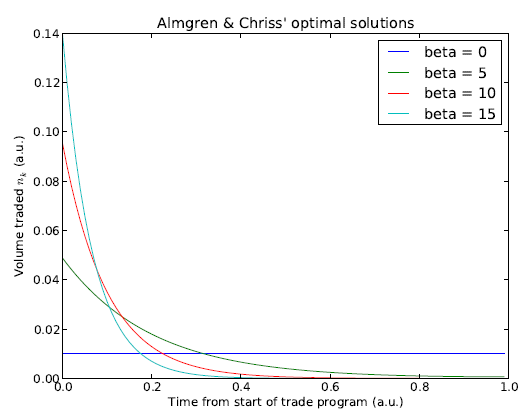
\includegraphics[width=0.7\textwidth]{picture/(7)AC_risk_averse.png}
\end{center}
\section{Almgren and Chriss continuous time}
The limitation of discrete model is:
\begin{itemize}
	\item Non-linear temporary impact
	\item Non-linear permanent impact
	\item Benchmarks different from IS
	\item Utility function instead of mean-variance optimization
	\item Static vs dynamic strategies
	\item Multiple assets
\end{itemize}
to handle these, we use continuous setting
\newpage
\begin{mysetting}[AC in continuous time]
	\begin{itemize}
		\item Sell $q_0$ shares, $dq_t = v_tdt$
		\item Set of admissible strategies:
		\[
		\mathcal{A} = \left\{ (v_t)_{t \in [0,T]}: \int_{0}^{T}v_td_t = -q_0 ; \int_{0}^{T}|v_t|dt \text{ a.s. bounded }rv \right\}
		\]
		\item $dS_t = \sigma dW_t + kv_tdt$
		usually price is given by geometric brownian motion, in this setting we have choosen arithmetic one because is easier and in intra-day arithmetic $\sim$ geometric
		\item $V_td_T$ volume traded by other agents is $[t,t+dt]$: we consider it deterministic, continuous, positive and bounded
		\item $X_t$ cash account:
		\[
		dX_t = -v_t \left(S_t + g\left(\frac{v_t}{V_t}\right)\right)dt = -v_tS_tdt + V_t L\left(\frac{v_t}{V_t}\right)dt
		\]
		here we consider $L(\rho) \equiv \rho g(\rho)$ s.t. $L(0) =0$, it is convex and $\lim_{\rho \to + \infty} = \frac{L(\rho)}{\rho} = +\infty$. For AC we consider:
		\[
		L(\rho) = \eta \rho^2
		\]
	\end{itemize}
\end{mysetting}
\begin{mytheorem}[Permanent impat is linear in AC like model]
	Given the model (no temporary impact):
	\[
	\begin{cases}
		& dq_t = v_t dt\\
		& S_t = \sigma dW_t + f(v_t)dt\\
		& dX_t = -v_tS_Tdt
	\end{cases}
	\]
	there is a dynamic arbitrage if there exists $(v_t)_t$ and $t_1<t_2$ s.t:
	\begin{align}
		&\int_{t_1}^{t_2} (|v_t| + |f(v_t)|)dt \in L^{\infty} (\Omega) \qquad (\text{boundedness})\\
		&\int_{t_1}^{t_2}v_tdt = 0 \quad \text{exist a round-trip: buy and sell same quantity]}\\
		&\expected{X_{t_2}|\mathcal{F}_{t_1}}>X_{t_1} \quad (\text{dynamic arbitrage})
	\end{align}
In words: exist a round trip strategy that is profitable on average
\end{mytheorem}
Let us introduce the utility function.
\begin{mydefinition}[Utility function]
	There exists an increasing and concave function $u(x)$ (utility function) such that a lottery $X$ (real-valued random variable modeling the outcome of the gamble) is prefered to a lottery $Y \iff \expected{u(X)} \geq \expected{u(Y)}$  
\end{mydefinition}
\begin{mytheorem}[Jensen inequality]
	If $u$ is concave, than:
	\[
	\expected{u(X)} \leq u(\expected{X})
	\]
\end{mytheorem}
\begin{mydefinition}[Absolute risk aversion function]
	Let $u$ be a twice differentiable utility function s.t. $u'>0$. We define the absolute risk aversion $\gamma(x)$ as:
	\[
	\gamma(x) = -u''(x)/u(x)
	\]
	which is invariant by increasing affine transformation of $u$
\end{mydefinition}
\begin{mydefinition}[Constant absolute risk aversion (CARA)]
CARA utility function is $u(x)$ s.t. $\gamma(x)$ is constant, so:
\[
u(x) = -\exp(-\gamma x)
\]
for $\gamma >0$ and $u(x) =x$ for $\gamma = 0$
\end{mydefinition}
\begin{mydefinition}[CRRA utility function]
CRR utility function is:
\[
u(x)= x^{1-\rho}/(1-\rho)
\]
if $\rho \to 1$:
\[
u(x) = \log x
\]
\end{mydefinition}
\newpage
\begin{mytheorem}[Expected value CARA function]
	Let $X$ be a real-valued Gaussian random variable $N(\mu, \sigma^2)$. Let $\gamma >0$, then:
	\[
	\expected{-\exp(-\gamma X)} = -\exp\left(-\gamma \mu + \frac{1}{2}\gamma^2\sigma^2\right)
	\]
\end{mytheorem}
\begin{mydefinition}[Cetainity equivalent]
	Let $u$ be a continuous and increasing utility function. Let $X$ be a real-valued random variable s.t. $X,u(X) \in L^1(\Omega)$. The certainty equivalent of $X$ for utility function $u$ is the unique $e\in \mathbf{R}$ s.t.:
	\[
	\expected{u(X)}=u(e)
	\]
	The certainty equivalent of a lottery is the risk-free payoff that has the same expected utility as the lottery.
If utility function is CARA with absolute risk aversion $\gamma$, the certainity equivalent is:
\[
e = \mu - \frac{1}{2}\gamma\sigma^2
\]
\end{mydefinition}
\begin{mysetting}[Deterministic strategies]
	Let us assume CARA risk averse investor, we have to maximize:
	\[
	\expected{-\exp(-\gamma X_T)}
	\]
If we restrict to deterministic strategies:
\[
\mathcal{A}_{det} = \left\{ (v_t)_{t \in [0,T]} \in \mathcal{A}, \forall t \quad v_t \text{ is } \mathcal{F}_0 - \text{measurable} \right\}
\]
Terminal cash is:
\[
X_t = X_0 + q_0S_0 - \frac{k}{2}q_0^2 + \sigma \int_{0}^{T}q_tdW_t - \int_{0}^{T}V_t L \left(\frac{v_t}{V_t}\right)dt
\]
assuming $c_t \in \mathcal{A}_{det}, X_t \sim \mathcal{N}(\mu_x,\sigma^2_X)$, than:
\begin{align*}
&\mu_x = X_0 + q_0S_0 - \frac{k}{2}q_0^2 - \int_{0}^{T} V_t L\left(\frac{v_t}{V_t}\right)dt\\
& \sigma_X^2 = \sigma^2 \int_{0}^{T} q^2_t dt
\end{align*}
\end{mysetting}
Let consider two cases:
\begin{itemize}
	\item $\gamma=0$(risk neutral investor), $\expected{X_T} = \mu_X$, can be minimized by $v_t \propto V_t$ due to convexity of $L$ (due to Jensen inequality)
	\item $\gamma>0$(risk averse investor) we can use Laplace trasform of the Gaussian and the problem can be rewritten as the minimization of the function $q(t)$:
	\[
	J(q) = \int_{0}^{T} \left(V_tL\left(\frac{q'(t)}{V_t}\right) + \frac{\gamma}{2} \sigma^2 \int_0^T q^2(t) dt\right)dt
	\]
	in the set $\mathcal{C}$ of absolutely continuous functions $q(t)$ in $[0,T]$ with $q(0) =q_0$ and $q(T)=0$.\\
	This problem is known as Bolza problem
\end{itemize} 
\begin{mytheorem}[Existing unique minimizer Bolza problem]
	There exists a unique minimizer $q^*$ of the function $J$ over the set $\mathcal{C}$, $q^*$ is a monotone funciton:
	\begin{itemize}
		\item if $q_0\geq 0$, $q^*$ is a nonincreasing function of time
		\item if $q_0\leq 0$, $q^*$ is a nondecreasing function of time
	\end{itemize}
In word: I cannot have a mixing buy-selling strategies
\end{mytheorem}
\subsection{Lagrangian setting}
We can translate this optimization problem in a Hamiltonian setting; Hamiltonian equations are:
\[
\begin{cases}
	 p'(t) = \gamma \sigma^2 q(t)\\
	 q'(t) = V_t H'(p(t))\\
	 q(0) = q_0\\
	 q(T) = 0
\end{cases}
\]
Where $H$ is the Legendre-Frenchel transform:
\[
H(p) = \sup_{\rho} \rho p - L(\rho)
\]
If L has continuous first two partial derivatives wrt all its arguments, one can introduce the Lagrangian:
\[
\mathcal{L}(t,q(t),q'(t))=V_t L\left(\frac{q'(t)}{V_t}\right) + \frac{\gamma}{2} \sigma^2 q^2(t)
\]
and using Eular-Lagrande equation:
\[
\frac{\partial \mathcal{L}}{\partial q} - \frac{d}{dt} \frac{\partial \mathcal{L}}{\partial q'} = 0
\]
with bounday conditions: $q(0) =q_0$ and $q(T) = 0$
\newpage
\begin{mytheorem}[Lagrange solution AC setting]
In AC setting, $L(\rho) = \eta \rho^2$, than $H(p) = \frac{p^2}{4 \eta}$, using Hamiltonian system and Euler-Langrange equation, we obtain:
\[
q''(t) = \frac{\gamma \sigma^2 V_t}{2 \eta}q(t)
\]
Special case $V_t = V$, solution is:
\[
q^*(t) = q_0 \frac{\sinh \left(\sqrt{\frac{\gamma \sigma^2 V}{2 \eta}}(T-t)\right)}{\sinh \left(\sqrt{\frac{\gamma \sigma^2 V}{2 \eta}T}\right)}
\]
solution doesn not depend on impact coefficient $k$
\end{mytheorem}
\begin{center}
	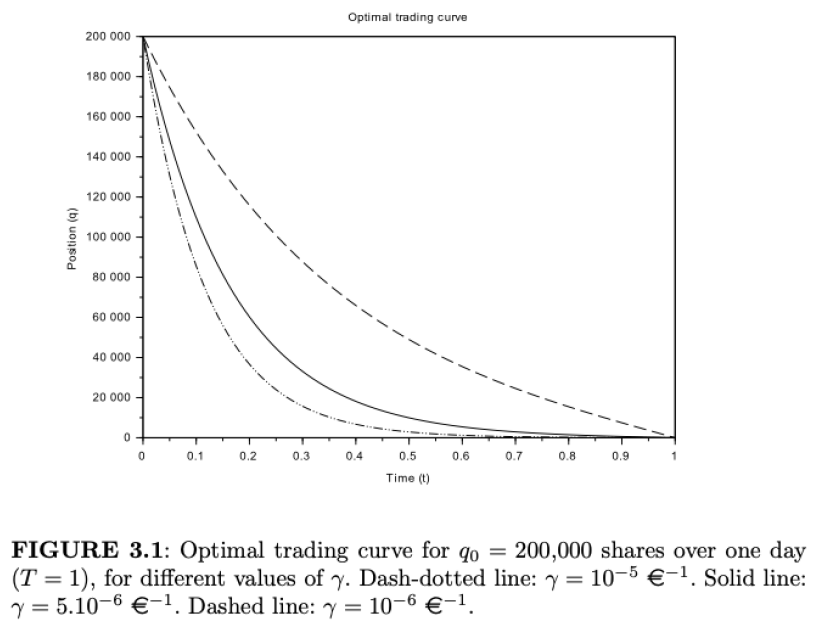
\includegraphics[width=0.5\textwidth]{picture/(8)AC_optimal_solution.png}
\end{center}
Let us analyse Stochastic strategies:
\begin{mytheorem}[Stochastic Strategies ]
	\[
	\sup_{v \in \mathcal{A}} \expected{-\exp({-\gamma X_T})} = \sup_{v \in \mathcal{A}_{det}} \expected{- \exp(-\gamma X_T)}
	\]
In CARA case, stochastic case does not have advantage on deterministic
\end{mytheorem}
Adding a participation rate constraint:
\[
\mathcal{A}_{\rho_\text{max}} = \left\{(v_t)_{t \in [0,T]} \text{prog. meas:} \int_{0}^{T} v_t dt = -q_0; |v_t| \leq \rho_{\max}V_t\right\}
\]
We can use a trick in order to solve this problem: constraintthe objective function
\[
J(q) = \int_{0}^{T} \left(V_tL_{\rho_{\max}}\left(\frac{q'(t)}{V_t}\right) + \frac{\gamma}{2} \sigma^2 \int_0^T q^2(t) dt\right) dt 
\]
where:
\[
L_{\rho_{\max}} = \begin{cases}
	 L(\rho) & |\rho| \leq \rho_{\max}\\
	+\infty & |\rho| > \rho_{\max}
\end{cases}
\]
\begin{mytheorem}[Solution AC adding participation rate constraint]
	There exists a unique minimizer $q^*$ of the functional $J$ over the set $\mathcal{C}$. If $q_0 \geq 0$, then $q^*$ is a nonincreasing function of time. If $q_0\leq 0$, then $q^*$ is a nondecreasing function of time. Furthermore, $q^*$ is uniquely characterized by:
	\[
	\begin{cases*}
		p'(t) = \gamma \sigma^2 q(t) 	\\
		q'(t) = V_t H'_{\rho_{\max}}(p(t))\\
		q(0) = q_0\\
		q(T) = 0 
	\end{cases*}
	\]
where $H_{\rho_{\max}}$ is the Legendre-Frenchel transform:
\[
H_{\rho_{\max}}(p) = \sup_{|\rho| \leq \rho_{\max}} \rho p - L(\rho)
\]
\end{mytheorem}
Let us discretization the Hamiltonian system: if $t_0 = 0 < \ldots < t_n = n\tau < \ldots<t_N = N\tau = T$, the discretized system is:
\[
\begin{cases}
	p_{n+1} = p_n + \tau \gamma \sigma^2 q_{n+1}, & 0\leq n<N-1\\
	q_{n+1} = q_n + \tau V_{n+1}H'(p_n), & 0 \leq n<N\\
	q_0 = q_0\\
	q_N = 0
\end{cases}
\]
We can solve this problem through fixed-point approach:
\[
\begin{cases}
	p_{n+1}^{\lambda} = p_n^{\lambda} + \tau \gamma \sigma^2 q_{n+1}^{\lambda}, & 0\leq n<N-1\\
	q_{n+1}^{\lambda} = q_n^{\lambda} + \tau V_{n+1}H'(p_n^{\lambda}), & 0 \leq n<N\\
	q_0^{\lambda} = q_0\\
	q_N^{\lambda} = 0
\end{cases}
\]
can be solved through bisection.
\newpage
\subsection{AC multi-asset portfolio}
\begin{mysetting}[AC model for a multi-asset portfolio]
If a trader wants to trade simultaneously a set of $d>1$ assets:
\begin{itemize}
	\item \textbf{Number of shares} $q_t^i = q_0^i - \int_{0}^{t}v_s^ids$
	\item \textbf{Price} $dS_t^i = \sigma^i dW_t^i - k^i v_t^idt$. $\Sigma$ is the covariance matrix of $\{ \sigma^i W_t^i\}$
	\item \textbf{Cash} $dX_t = \sum_{i=1}^{d} v_t^i S^i_t dt -V_t^i L^i \left(\frac{v_t^i}{V_t^i}\right)dt$
\end{itemize}
There is no cross-impact term, but the "interaction" between stocks is only through the covariance of prices.
\end{mysetting}
The value of terminal cash is:
\begin{align*}
	X_T & = X_0 + \sum_{i=1}^{d} q_0^i S_0^i - \sum_{i=1}^{d} \frac{k_i}{2}(q_0^i)^2 \\
	& + \sum_{i =1}^{d} \int_{0}^{T} q_t^i \sigma^i dW^i_t - \sum_{i=1}^{d} \int_0^T V_t^i L^i \left(\frac{v_t^i}{V_t^i}\right)dt
\end{align*}
The optimization problem is:
\[
\sup_{(v_t)_t \in \mathcal{A}} \expected{- \exp(-\gamma X_T)}
\]
As in the single-asset case, deterministic strategies are optimal.\\
Using Hamiltionian setting, minimization problem is:
\[
J(q) = \int_{0}^{T} \left(\sum_{i=1}^{d} V_t^i L^i \left(\frac{(q^i(t))'}{V_t^i}\right)  + \frac{\gamma}{2} q(t) \cdot \Sigma q(t)\right)
\]
Hamiltonm equation:
\[
\begin{cases}
	p'(t) = \gamma \Sigma q(t)\\
	(q^i(t))' = V_t^i (H(p^i(t)))'\\
	q(0) = q_0\\
	q(T) = 0	
\end{cases}
\]
with
\[
H^i (p) = \sup_{\rho} \rho p - L^i(\rho)
\]
\subsection{Hedging a liquidation with optimal execution of another asset}
A trader could want to mitigate the risk linked to the execution process by introducing a second asset correlated with the first one. This approach involves solving a multi-asset liquidation problem, starting with an initial position of $(q_0, 0)$. For instance, we can assume the presence of another asset denoted by the subscript "h" that has no associated execution costs, such as a futures contract.\\
The problem now is to minimize the functional:
\[
J(q(t),q_h(t)) = \int_{0}^{T} \left(V_t L \left(\frac{q'(t)}{V_t}\right) + \frac{\gamma}{2}\left(\sigma^2q^2(t) + 2 \rho \sigma \sigma_h q(t) q_h (t) + \sigma^2q_h^2(t)\right)\right)dt
\]
The optimal hedge consist in setting $q_h(t) = -\rho \frac{\sigma}{\sigma_h}q(t)$, and minimize the functional:
\[
\tilde{J}(q(t)) = J\left(q(t), - \rho \frac{\sigma}{\sigma_h}q(t)\right) = \int_{0}^{T} \left(V_t L \left(\left(\frac{q'(t)}{V_t}\right)\right) + \frac{\gamma}{2} \sigma^2 (1 - \rho^2)q^2(t)\right)dt
\]
\begin{center}
	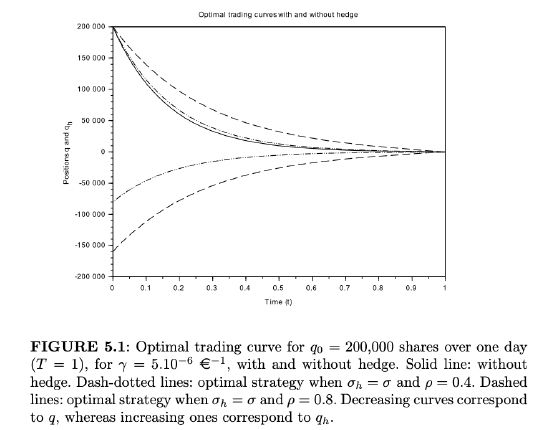
\includegraphics[width=0.5\textwidth]{picture/(9)AC_optimal_hedge.png}
\end{center}
Second asset perform a round trip, by building an initial position instantaneously and liquidating it progressively with an optimal trading curve given by: $q_h(t) = - \rho \frac{\sigma}{\sigma_h}q(t)$
\subsection{Case Percentage of Volume (POV)}
Changing set of admissible controls as:
\[
\mathcal{A}_{POV} = \left\{(v_t)_{t \in \mathbb{R}^+}, \exists \rho > 0, \forall t \geq 0, v_t = -\rho V_t \mathbf{1}_{\{\int_{0}^{t} \rho V_s ds \leq q_0\}}\right\}
\]
The terminal cash is:
\[
X_T = q_0S_0 - \frac{k}{2}q^2_0 - \frac{L(\rho)}{\rho}q_0 + \sigma \rho \int_{0}^{T} \int_{t}^{T} V_s dsdW_t
\]
which is a Gaussian random variable.\\
The expected utility can be obtained using a Laplaca transformation, the function to minimize is:
\[
J_{POV}(\rho) = \frac{L(\rho)}{\rho}q_0 + \frac{\gamma}{2} \sigma^2 \rho^2 \int_{0}^{T} \left(\int_t^T V_s ds\right)^2dt
\]
\begin{mytheorem}[Existence global minimum case POV]
	There exists a $\rho^*>0$ such that $J_{POV}$ has a glbal minimium
\end{mytheorem}
If $V_t = V$, than:
\[
J_{POV} = \frac{L(\rho)}{\rho}q_0 + \frac{\gamma}{6}\sigma^2 \frac{q_0^3}{\rho V}
\]
If $L(\rho) = \eta |\rho|^{1+ \phi} + \psi |\rho|$, optimal solution is:
\[
\rho^* = \left(\frac{\gamma \sigma^2}{6 \eta \phi}\frac{q_0^2}{V}\right)^{\frac{1}{1 + \phi}}
\]
The execution time will be fixed by $T^* = \frac{q_0}{V \rho^*}$. Some considerations:
\begin{itemize}
	\item $\rho^*$ does not depend on permanent impact and spread parameter $\psi$
	\item $\rho^*$ increases with risk aversion, volatility, inventory
	\item $\rho^*$ decreases with illiquidity $(\eta)$ and $\phi$
\end{itemize}
Through $\rho^*$, we can estimate the risk aversion $\gamma$ of a trader from its executions:
\[
\gamma = \frac{6 \eta \phi V(\rho^*)^{1+ \phi}}{\sigma^2 q_0^2}
\]
\section{Optimal execution with transient market impact}

Almgren and Chriss make an assumption of a market impact that is linear, fixed, and permanent. However, as discussed in previous lectures, due to the correlation of order flow, it is evident that market impact is not solely fixed and permanent; instead, it exhibits a transient nature. This means that the past order flow influences future price impacts. To account for this phenomenon, one approach is to use a transient impact model (TIM).\\
TIM assumes that:
\[
p_n = p_{-\infty} + \sum_{k=1}^{\infty}f(v_{n-k})G(k) + \sum_k \eta_k
\]
where $v_n$ is the signed order flow. So:
\[
p_{n+1} - p_n = G(1)f(v_n) + \sum_{k=1}^{\infty} [G(k+1) - G(k)]f(v_{n-k}) + \eta_n
\]
The decay of $G$ make price diffusive (or approximately efficient), given the correlated order flow.\\ The efficiency leads to:
\[
p_{n+1} - p_n = K(v_n - \hat{v}_n) + \eta_n
\]
where $\hat{v}_n$ is the best predictor of $v_n$ given $\mathcal{F}_n$\\
Let consider the propagator model in real time. We consider 5 minute intervals, $p_n$ is the log mid price right before time $t_n$. We define the series of aggregated volume $v_n$ in terms of the volume $v_i^{tt}$ of single transaction:
\[
v_n = \sum_{[t_n, t_{n+1}]} v_i^{tt}
\]
with $v_i = \sum \text{buy} - \sum \text{sell}$.\\
Consider the normalized volume imbalance:
\[
v_n^{nor} = \frac{\sum_{[t_n,t_{n+1}]} v_i^{tt}}{\sum_{[t_n,t_{n+1}]} |v_i^{tt}|}
\]
The impact function $f(v^{nor})$ of the normalized volume imbalance is:
\[
f(v^{nor}) = \expected{r_n| v_n^{nor}}
\]
and the propagator model in real time is:
\[
r_j \equiv p_{k+1} - p_k = \sum_{k=0}^{j-1} \mathcal{G}(k) f(v_{j-k}^{nor}) +\eta_j \qquad \mathcal{G}(k) \equiv G(k+1) -G(k), G(0) = 0
\]
\begin{center}
	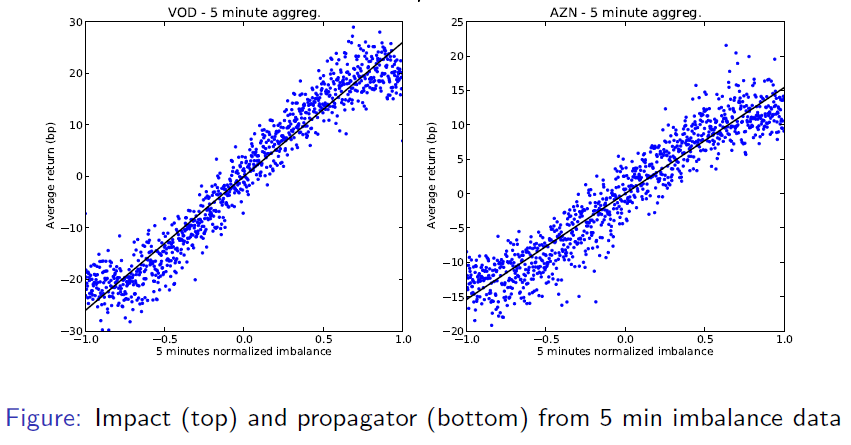
\includegraphics[width=0.5\textwidth]{picture/(10)market_impact_1.png}
\end{center}
We noticed that at this level of aggragation, impact is roughly linear.\\
Considering a different aggregations (number of trades):
\begin{center}
	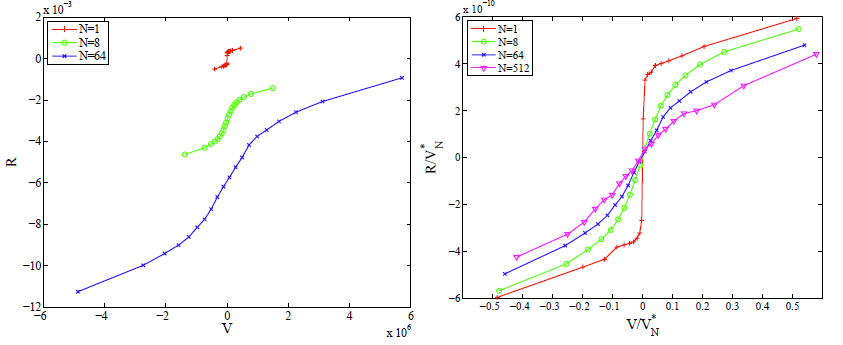
\includegraphics[width=0.5\textwidth]{picture/(11)market_impact_2.png}
\end{center}
Market impact is a strongly concave function of volume at short scales, but it becomes progressively more linear on longer scale.
\begin{center}
	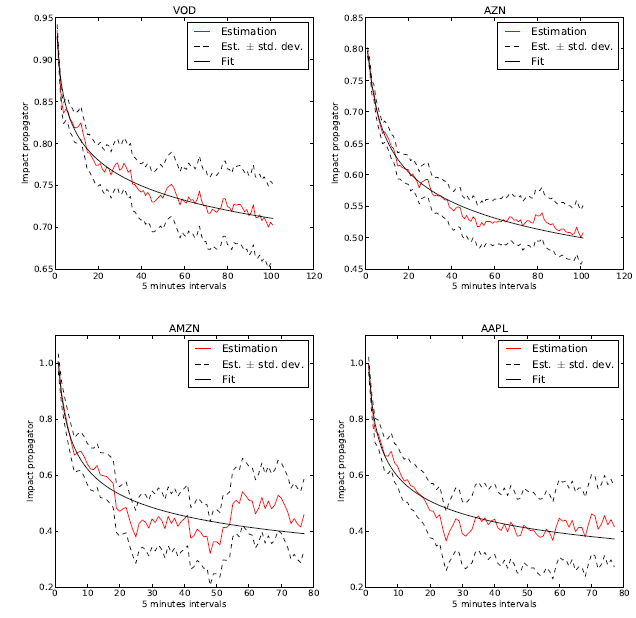
\includegraphics[width=0.5\textwidth]{picture/(12)market_impact_3.png}
\end{center}
The TIM fits data quite well also on aggregated (time or trades) data.\\
Considering optimal execution, effective $\log$-midprice $\tilde{p}_k$ is the logarithm of the average mid-price at which we trade the shares $v_k$ between time $t_k$ and time $t_{k+1}$, we assume:
\[
\tilde{p}_k = \frac{p_k + p_{k+1}}{2}
\]
the equation that describes the dynamics of effective price is:
\[
\tilde{p}_n = p_0 + \sum_{k=0}^{n} [\eta_k + f(v_k) \tilde{G}(n-k)]
\]
we degine effective propagator $\tilde{G}$ as:
\[
\tilde{G}(0) = \frac{G(1)}{2}, \quad \tilde{G}(1) = \frac{G(1) + G(2)}{2}, \quad \tilde{G}(2) = \frac{G(3)+G(2)}{2}, \ldots
\]
we define the logarithmic transiction cost $c(\mathbf{v})$ as:
\[
c(\mathbf{v}) \equiv \sum_{k=0}^{N-1} v_k (\tilde{p}_k - p_0) \simeq \sum_{k=0}^{N-1} v_k \log \left(\frac{\tilde{P}_k}{P_0}\right) \simeq \sum_{k=0}^{N-1}v_k \left(\frac{\tilde{P}_k - P_0}{P_0}\right) = \frac{C(\mathbf{v})}{P_0}
\]
The expected implementation shortfall is:
\[
\expected{C(\mathbf{v})} = \sum_{n=1}^{N}v_n \left[\sum_{k=1}^{n} f(v_k) \tilde{G}(n-k)\right]
\]
if we assyme instantaneous impact linear: $f(v_k) = \theta_kv_k$, we obtain:
\[
\expected{C(\mathbf{v})} = 2\sum_{k,j}\theta_k \tilde{G}(|k-j|) v_kv_j = \mathbf{v}^T\mathcal{I}\mathbf{v}
\]
where $\mathcal{I}$ is Toeplitz matrix.\\
In this way we obtain a quadratic optimization problem:
\[
\textbf{v}^* = \text{arg}\min_{v} \mathbf{v}^T\mathcal{I}\mathbf{v}, \quad \text{s.t.} \quad \sum_k v_k = \textbf{1}^T\textbf{v} = q_0
\]
solving through Lagranfe multiplier:
\[
\textbf{v}^* = \frac{q_0}{\mathbf{1}\mathcal{I}^{-1}\mathbf{1}}\mathcal{I}^{-1}\mathbf{1}
\]
If $G(k) = a(c+k)^{-\beta} \sim k^{-\beta}$
\begin{center}
	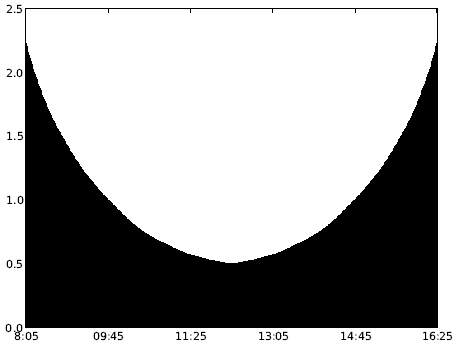
\includegraphics[width=0.4\textwidth]{picture/(13)solution_u_term.png}
\end{center}
The solution is symmetric around $N/2$. U shape does not depend on the intraday profile of volume.\\
\subsection{Adding risk term}
The variance of the execution cost under the propagator model is:
\begin{align*}
	Var[c(\textbf{v})] &= \expected{(c(\textbf{v}) - \expected{c(\textbf{v})})^2} = \expected{\left(\sum_{k=1}^{N}v_k \sum_{j=0}^{k-1} \eta_j\right)^2}=\\
	&= \expected{\left(\sum_{k=1}^{N}\eta_k \sum_{j=k}^N v_j\right)^2} = \sigma^2 \sum_{k=1}^N \left(\sum_{j=k}^N v_j\right)^2 = \sum_{k,j} \mathcal{V}_{k,j}v_kv_j
\end{align*}
where $\sigma^2$ is variance of the residuals. Defining $\mathcal{F} \equiv \mathcal{I} + \lambda \mathcal{V}$, using Lagrange myltipliers we define:
\[
\mathbf{v}^* = z \mathcal{F}^{-1} \mathbf{1} = \frac{q_0}{\mathbf{1}^T\mathcal{F}^{-1}\mathbf{1}}\mathcal{F}^{-1}\mathbf{1}
\]
Plotting it, more is risk adversion, more trading at begging:
\begin{center}
	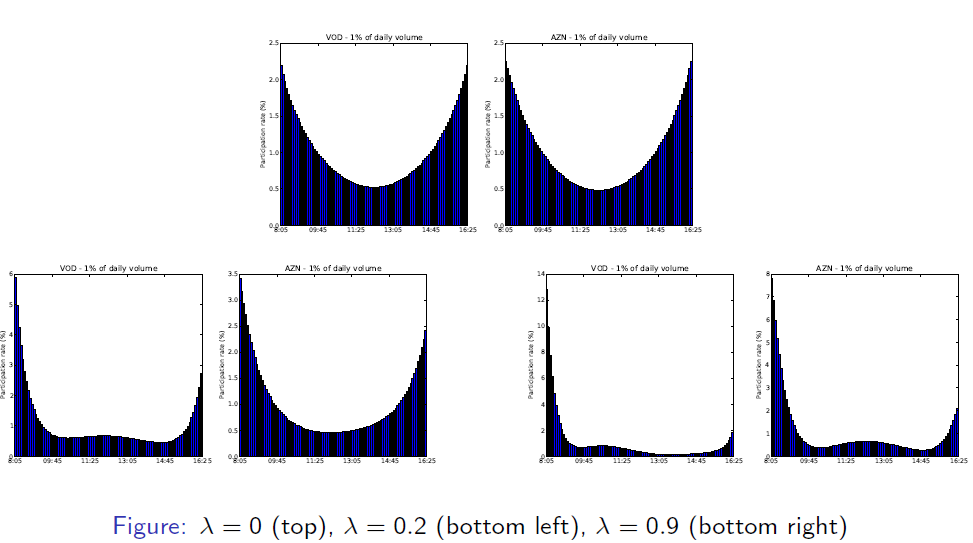
\includegraphics[width=0.6\textwidth]{picture/(14)solution_u_term_risk.png}
\end{center}
\subsection{Including spread costs (no risk aversion)}
In this derivation, we have not included transiction cost (fees, spread), spread costs change the qualitative results more.\\
Model price is:
\[
\tilde{p}_n = p_0 + \sum_{k=0}^{n} [\eta_k + f(v_k) \tilde{G}(n-k)] + \text{sign}(v_k)\delta_k
\]
so that we payy half the bid-ask spread ib execution, we have defined:
\[
\delta_k \equiv \frac{s_k/2}{P} = \frac{A_k-B_k}{A_k+B_k}
\]
with $A,B$ ask-bid spread. The objective function to optimize is:
\[
F[\textbf{v}] = \expected{C(\textbf{v})} + Spread(\textbf{v}) = \textbf{v}^T \mathcal{I}\textbf{v} + \textbf{D}^T |\textbf{v}|
\]
with $\textbf{D} = (\{\delta_k\})^T$ is a vectore describing the spread cost during execution, for simplicity we assume $\textbf{D} = \delta \textbf{1}$. Solving it numerically, the shape of the solution does not qualitatively change.
\begin{center}
	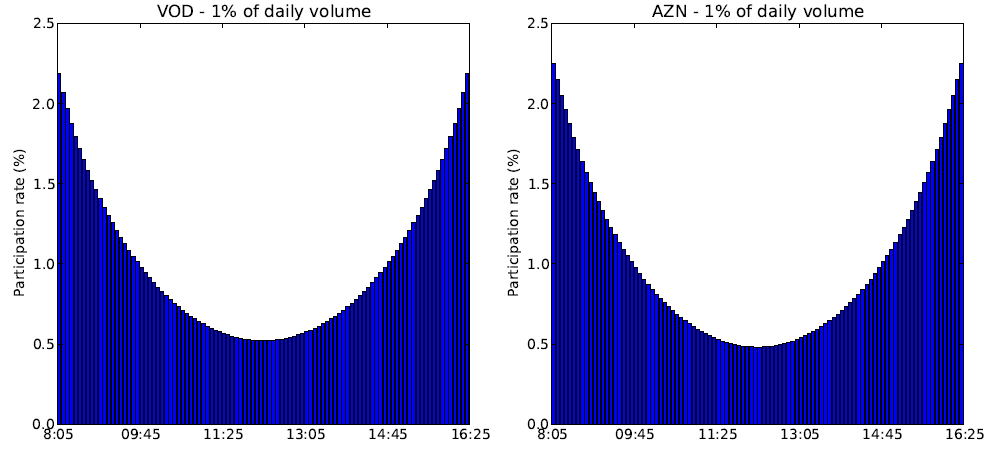
\includegraphics[width=0.6\textwidth]{picture/(15)solution_u_term_transiction.png}
\end{center}
General comments:
\begin{itemize}
	\item The alternating (buy-sell) solution and the regularization achieved by the bid ask
	term is similar to what happens in portfolio optimization.
	\item By choosing a $\delta$ parameter much smaller than the fractional spread, one still
	recovers the U-shaped solution.
\end{itemize}
\section{Transient Impact Model (TIM) in continuous time}
Considering time interval $[0,T]$, the price $S_t$ at time $t$ is:
\[
S_t = S_0 + \int_{0}^{t} f(\dot{q}_s) G(t-s)ds + \int_0^t \sigma_sdW_s 
\]
where $(\dot{q}_t)$ is the amount of shares sold by the execution time $[t,t+dt]$, $W_s$ is a Wiener process, $\sigma_s$ is deterministic function. The function $f$ describes the instantaneous impact of the executed trades on price, we consider it linear:
\[
f(\dot{q}_t) = -k \dot{q}_t
\]
The function $G(t)$ describes the delayed effect of trading on price and $G(t-s)$ characterizes how a trade at time $s$ affects the price at time $t$.\\
Empirical evidences, shows power law kernel:
\[
G(t) = t^{-\kappa},\quad \kappa<1
\]
\begin{mysetting}[TIM continuous generalized VWAP]
	\begin{itemize}
		\item borker receives from a fund a request of a VWAP sell execution of $q_0>0$ shares in a time windows $[T_1,T_2]$ termed the benchmark interval.
		\item The broker charges the fund the Volume Weighted Average Price in $[T_1,T_2]$.
		\item The broker is allowed to trade in a time window $[0,T] \supseteq [T_1,T_2]$
	\end{itemize}
\end{mysetting}
\begin{center}
	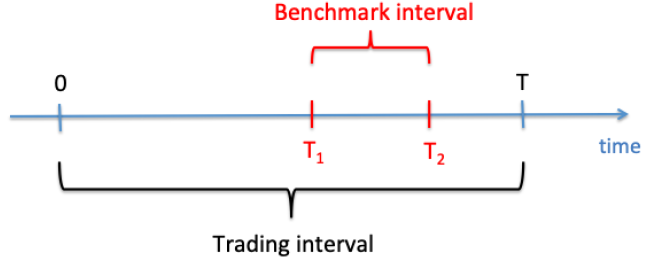
\includegraphics[width=0.6\textwidth]{picture/(16)setting_TIM_VWAP.png}
\end{center}
We will consider only deterministic strategies.\\
Let $V_tdt$ be the deterministic market volume traded in $[t,t+dt]$. VWAP benchmark is given by:
\[
VWAP_{T_1}^{T_2} = \frac{\int_{T_1}^{T_2} S_tV_t dt}{\int_{T_1}^{T_2} V_t dt} = \int_{0}^{T} \eta_t S_t dt
\]
where:
\[
\eta_t = \frac{V_t}{\int_{T_1}^{T_2}V_sds}\mathds{1}_{t\in [T_1,T_2]}
\]
The objective function of the broker is the difference between the cash she is able to obtain from the proceeds in the trading interval and the cash she will give back to the client, equal to the random variable $q_0VWAP_{T_1}^{T_2}$, let use define the cash process (no temporary impact):
\[
dX_t = \dot{q}_tS_tdt =v_tS_tdt\qquad X_0=0
\]
Assuming CARA risk averse agent, objective function is:
\[
U[\textbf{q}] = \begin{cases}
	\expected{X_T - q_0 q_0VWAP_{T_1}^{T_2}}& \gamma = 0\\
	\expected{-\exp(-2\gamma(X_T - q_0VWAP_{T_1}^{T_2}))} &\gamma >0
\end{cases}
\]
where $2\gamma$ is risk aversion parameter.
\begin{mytheorem}[Optimization problem TIM generalized VWAP]
	Under linear impact, $f(z) = -kz, k>0$, the maximization of the utility function over the deterministic strategies is equivalent to the minimization of the functional:
	\begin{align}
	C[\mathbf{x}]&\equiv \frac{1}{2} \int_{0}^{T} \int_0^T \dot{q}_t \dot{q}_s G(|t-s|)dsdt - q_0 \int_0^T \eta_t dt \int_0^t G(t-s) \dot{q}_s ds\\
	& + \frac{\gamma}{k}\int_0^T\int_0^T dt dt'(\dot{q}_t - q_0\eta_t)(\dot{q}_{t'} -q_0\eta_{t'})\int_0^{t \land t'} \sigma^2_sds
	\end{align}
\end{mytheorem}
This is not a standard Lagrangian calculus of variation, we need a different approach form Euler-Lagrange.\\
If $\gamma =0$, minimization is:
\[
C[\textbf{q}] = \frac{1}{2} \int_0^T \int_0^T dq_tdq_s G(|t-s|) - \frac{q_0}{T}\int_0^T dt \int_0^t G(t-s)dq_s \equiv Q[\textbf{q}] + K[\textbf{q}]
\]
Considering a strategy:
\[
dy_s = \delta_{t_2}(ds) - \delta_{t_1}(ds) \qquad 0\leq t_1 \leq t_2 \leq T
\]
Let call $\textbf{q}^*$ the optimal strategy, and setting $\textbf{z} = \textbf{q}^* + \alpha \textbf{y}$, the integral equation satisfied the optimal strategy:
\[
\frac{\partial \expected{C[\textbf{z}]}_0}{\partial \alpha}\Bigr|_{\alpha = 0} = 0
\]
\begin{mytheorem}[Integral equation associated to Optimization problem TIM generalized VWAP]
	The strategy $\{q_t^*\}^T_0$ thath minimize the functional (with $\gamma = 0$), satisfies the integral equation:
	\[
	\int_0^T G(|t-s|)dq^*_s - q_0 \int_t^T \eta_s G(s-t)ds = \lambda
	\]
where $\lambda$ is a constant set by the normalization the total volume traded:
\[
\int_0^T dq^*_s = q_0
\]
\end{mytheorem}
We write the solution of the integral equation as:
\[
w_s = \dot{q}_s^* - q_0\eta_s
\]
with $\int_0^T w_sds=0$, replacing it in integral equation:
\[
\int_0^T G(|t-s|) w_sds = \lambda - q_0 \int_0^t \eta_sG(t-s)ds
\]
writing the solutuon $w_s = w_s^{(1)} + w_s^{(2)}$, where the second tem solves:
\[
\int_0^T G(|t-s|)w_s^{(2)}ds = -q_0\int_0^t \eta_s G(t-s)ds
\]
and setting $q'_0 = \int_0^T w_s^{(2)}ds$, the first term solves:
\[
\int_0^T G(|t-s|)w_s^{(1)}ds = \lambda \qquad \int_0^T w_s^{(1)}ds = -q'_0
\]
which is the equation when the objective function is the IS and nu,ber of shares is $-q_0'$.
If $T_1 = T_2 = 0$, $\eta_t = 2\delta(t)$ and integral equation becomes:
\[
\int_0^T G(|t-s|)dq^*_s = \lambda
\]
\newpage
\begin{mytheorem}[Existence minimization value implementation Shortfall]
	Suppose $G$ is positive definite. Then $q^*$ minimizes expected cos $\iff$ $\exists\lambda$ s.t. $q_t^*$ solves $\forall t$:
	\[
	\int_0^T G(|t-s|)dq^*_s = \lambda
	\]
thus $C(q^*) = \frac{1}{2} \lambda q_0$
\end{mytheorem}
\subsection{Obizhaeva-Wang model}
\begin{mysetting}[Obizhaeva-Wang model]
	\begin{itemize}
		\item Impact is linear and decays exponentially in time
		\item The decay is interpreted as the relaxation of the limit order book when shocked by a trade
		\item so that $v_t = \dot{q}_t$, the price during the execution is modeled as:
		\[
		S_t = S_0 - k \int_0^T v_s \exp[-\rho(t-s)]ds + \int_0^t \sigma dW_t
		\]
	\end{itemize}
\end{mysetting}
The expected cost is:
\[
\expected{C[\mathbf{q}]} = k \int_0^T v_tdt \int_0^t v_s \exp[-\rho(t-s)]ds
\]
\begin{mytheorem}[Solution Obizhaeva-Wang model]
	The Fredholm integral equation of the first kind from the theorem is:
	\[
	\int_0^T v_s\exp[-\rho |t-s|]ds =\lambda
	\]
where $\lambda$ is integration constant. The exact solution is:
\[
v_t = (q_0 -\rho T) + \rho + (q_0 - \rho T)\delta(t-T)
\]
\end{mytheorem}
In special case $T_1 = T_2 = T$, integral equation is:
\[
\int_0^T G(|t-s|) dq_s^* = \lambda + q_0G(T-t)
\]
with solution $\dot{q}_s^* = w_s^{(1)} + q_0 \delta(T-t)$ (the sum of $q_0/2$ shares traded as in the IS case and the remaining $q_0/2$ shares traded at $t=T$).\\
Using power law kernel $G(t) = e^{-\rho t}$, the optimal strategy is:
\[
v_t = \frac{q_0}{\rho T (2+ \rho T)} [ 2(1 + \rho T)\delta(t) + \rho(1+ \rho T) - 2\delta (t-T)]
\]
in word: sell a finite amount at time $t=0$, selling at a constant rate for whole interval $(0,T)$, buying a finite amount at time $t=T$.
\section{Solution TIM in discrete time}
When we add more constraints, it is convenient to frame the problem in discrete time, we can make it at three different levels:
\begin{itemize}
	\item express the cost function in discrete time and solve the optimization;
	\item use discrete time to obtain a quadrature of the integral equation;
	\item write the Transient Impact Model in discrete time, derive the corresponding cost and then minimize it.
\end{itemize}
The three method does not give the same results, if time intervals for discretization is sufficiently small, differences become negligible. We will use the last setting.
\begin{mysetting}[TIM Discrete Time]
	\begin{itemize}
		\item Let us divide the interval $[0;T]$ in $N$ equal intervals and define $\tau = T/N$.
		\item The strategy is now a vector $\textbf{v} = (v_1,\ldots,v_N)'$, with $v_i$ we consider amount of shares traded in interval $i$
		\item The price dybamics of sell execution is:
		\[
		S_l = S_0 -k\sum_{i=1}^{l} G(l-i)v_i + \tau^{1/2} \sum_{i=1}^{l} \epsilon_l \qquad l = \{0,\ldots, N\}
		\]
		that can be rewritten as:
		\[
		\textbf{S} =S_0 \textbf{1} -kG \textbf{v}+ \tau^{1/2} L\epsilon
		\]
		where $\textbf{S} = (S_1,\dots,S_N)', \textbf{1} = (1,\ldots,1), L$ is lower triangular matrix of ones, $G$ is the lower triangular matrix s.t:
		\[
		G_{ij} = G[\tau(i-j)] \quad \text{if } i\geq j 
		\]
		and $\epsilon \sim \mathcal{N}(\mathbf{\mu},\mathbf{\Sigma})$ is Gaussian random vector describing the price dynamics.
	\end{itemize}
\end{mysetting}
Consider a $VWAP$ benchmark between $t=T_1$ and $t=T_2$, corresponding to $l_1 = \lfloor NT_1/T\rfloor$, $l_2 = \lfloor NT_2/T\rfloor$ are the rounding to the nearest integer. Introducing $B = \{l \in \mathbb{N}: l_1 \leq l \leq l_2 \}$ and a vector $\mathbf{\eta}$ with components:
\[
\eta_l = \frac{V_l}{||\eta||_1} \mathds{1}_{l \in B}
\]
where $V_l$ is the market colume traded in interval $l$.\\
The benchmark is $q_0\mathbf{\eta}'\mathbf{S}$, and normalization ensures that $\mathbf{1}'\mathbf{\eta} =1$.\\
We use utility function $\mathcal{U}[(\mathbf{v} - q_0 \mathbf{\eta})'\mathbf{S}]$ and using CARA utility function with risk aversion $2\gamma$, the expected utility is:
\[
U[\mathbf{x}] = \expected{(\mathbf{v} -q_0\mathbf{\eta})'\mathbf{S}}_0 - \gamma \mathbb{V}_0[(\mathbf{v}-q_0\mathbf{\eta})'\mathbf{S}]
\]
\begin{mytheorem}[Solution discrete TIM VWAP execution]
Under CARA utility function iwth risk aversion $2\gamma$, the optimal VWAP execution which maximizes the expected utility, is the solution of the quadratic optimization
\[
\min_{v}[\mathbf{v}'A\mathbf{v} - \mathbf{b}'\mathbf{v}] \qquad \text{s.t.} \mathbf{1}'\mathbf{v}=q_0
\]
where:
\begin{align}
&A =kG + \gamma \tau L \Sigma L'\\
&\mathbf{b}' = kq_0 \mathbf{\eta}'G + 2\gamma \tau q_0 \mathbf{\eta}'L\Sigma L' + \tau^{1/2} \mathbf{\mu}' L'
\end{align}
The matrix $A$ is positive and definite if $\Sigma$ is positive definite. The solution of the quadratic optimization exists and is unique.
\end{mytheorem}
Due to quadratic form, several constraints can be added:
\begin{center}
	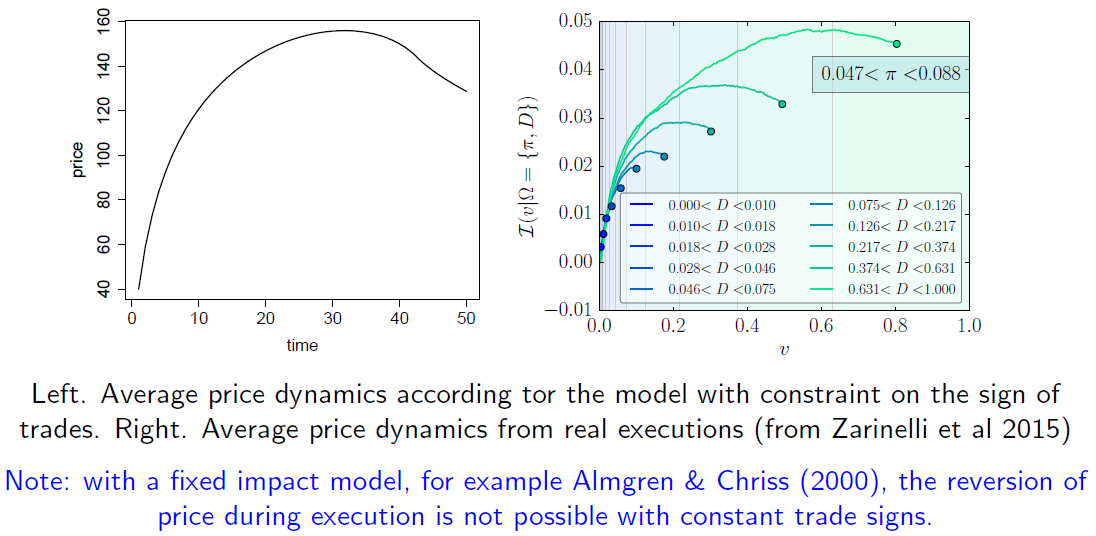
\includegraphics[width=0.6\textwidth]{picture/(17)TIM_discrete_1.png}
\end{center}
\begin{center}
	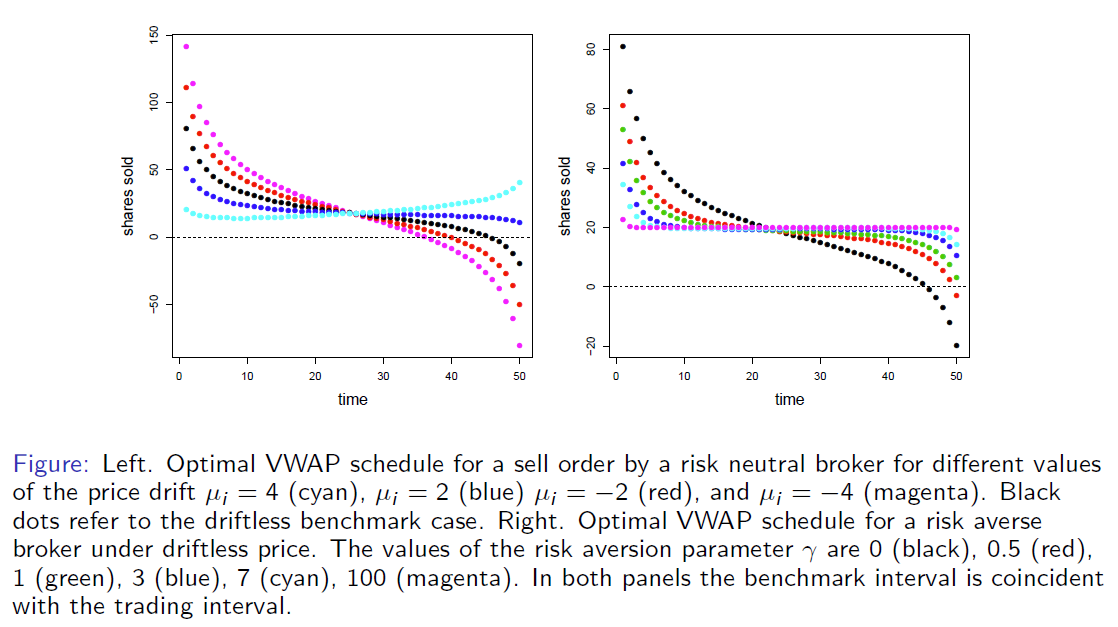
\includegraphics[width=0.6\textwidth]{picture/(18)TIM_discrete_2.png}
\end{center}
\begin{center}
	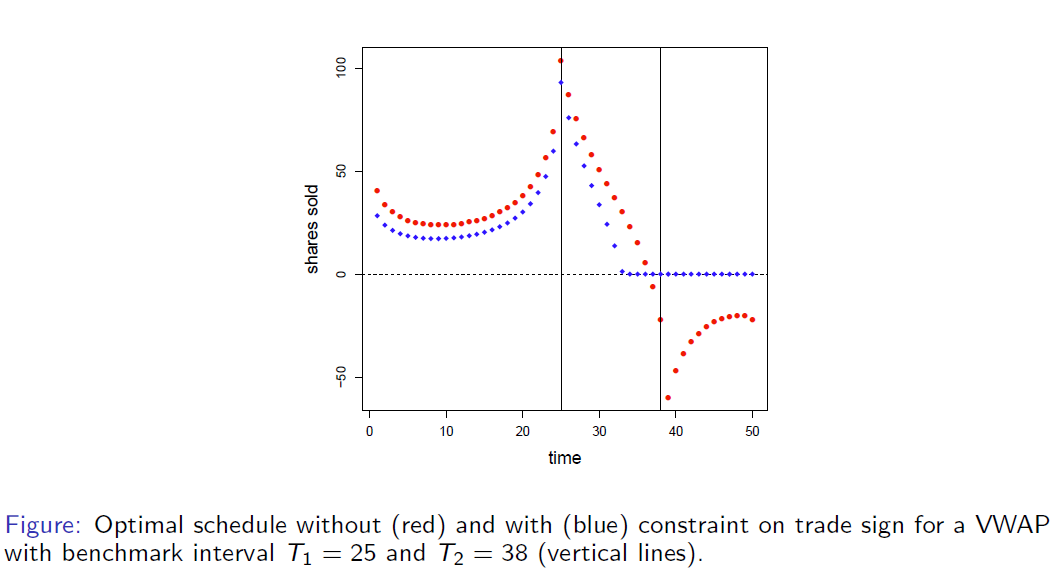
\includegraphics[width=0.6\textwidth]{picture/(19)TIM_discrete_3.png}
\end{center}
From this picture we can notice the strategy is: selling a lot in the begging to buy in the end.
\section{Price manipulation}
Let us define:
\begin{itemize}
	\item $q_0$ shares to be sold
	\item $S_t^0$= unperturbed price; $S_t^q =$ price when strategy $q$ is used
	\item Revenues:
	\[
	\mathcal{R}_T(q) = -\int_0^T S_t^qdq_t
	\]
	\item Liquidation cost:
	\[
	\mathcal{C}_T(q) = q_0S_0^0 - \mathcal{R}_T(q)
	\]
both stochastic.
\item $dq_t$: number of shares traded in $[t,t+dt]$
\end{itemize}
\begin{mydefinition}[Price manipulation]
	A round trip is an order execution strategy $(q_t)_{t \in [0,T]}$ with $q_0 =q_t =0$. A price manipulation strategy is a round trip with:
	\[
\expected{\mathcal{R}_T(q)}>0	
	\]
\end{mydefinition}
\begin{mydefinition}[Transaction-triggered price manipulation (Alfonsi et al 2012)]
	A market impact model admits transaction-triggered price manipulation if the expected revenues of a sell (buy) program can be increased by intermediate buy (sell) trades. In other words, $\exists q_0,T>0,\tilde{q}$, s.t.":
	\[
	\expected{\mathcal{R}_T(\tilde{q})} > \sup \{\expected{\mathcal{R}_T(q)}\}\quad q \text{ is monotone}
	\]
\end{mydefinition}
\begin{mydefinition}[Negative expected liquidation]
	A market impact model has negative expected liquidation costs if
	\[
	\expected{\mathcal{C}_T (q)} <0
	\]
or $\expected{\mathcal{R}_T (q)} > q_0S_0$
\end{mydefinition}
\begin{mytheorem}[Relation between manipulations (Kl\"{o}ck et all 2011)]
	\begin{itemize}
		\item Any market impact model that does not admit negative expected liquidation costs does also not admit price manipulation.
		\item Suppose that asset prices are decreased by sell orders and increased by buy orders.
		Then the absence of transaction-triggered price manipulation implies that the model
		does not admit negative expected liquidation costs. In particular, the absence of
		transaction-triggered price manipulation implies the absence of price manipulation in
		the usual sense.
	\end{itemize}
\end{mytheorem}
Let consider AC model: gicen two non-decreasing functions $f$ and $g$, with $f(0) =g(0) = 0$, an absolutely contionuous strategy $(q_t)_{t\geq 0}$ leads to a price trajectory:
\[
S^q_t = S^0_t + \int_0^t \underbrace{f(\dot{q}_s)ds}_{\text{permanent price impact}} + \underbrace{g(\dot{q}_s)}_{\text{temporary-impact}}
\]
assuming:
\[
S_t^0 =S_0 + \sigma W_t
\]
and $W_t$ is a Wiener process
\begin{mytheorem}[AC model price manipulation (Huberman and Stanzl 2004, Gatheral 2010)]
	If the AC model does not admit price manipulation, then $f(x)=\gamma x$ with $\gamma \geq 0$
\end{mytheorem}
This theorem show that non-linear permanent market impact is inconsistent with the principle of no price manipulation.
\subsection{Transient impact models}
Empirical evidences shows that the impact is transient (decay with time). We can generalize the TIM model as:
\[
S_t^q = S_0 + \int_0^T f(\dot{q}_s)G(t-s)ds + \int_0^t \sigma dW_s
\]
with expected cost:
\[
\expected{\mathcal{C}_T(q)} = \int_0^T \dot{q}_tdt + \int_0^t f(\dot{q}_s)G(t-s)ds
\]
\begin{mytheorem}[Non-linear Obizhaeva-Wang model manipulation]
Considering:
\[
S_t^q = S_0 + \eta \int_0^T f(v_s)\exp[-\rho (t-s)] ds + \int_0^t \sigma dW_t
\]
If the temporary market impact decays exponentially, then price manipulation is possible unless $f(v)\propto v$
\end{mytheorem}
If we assume the instantaneous impact is linear $f(v) = \gamma v$, then:
\begin{align*}
	&S_t^q = S_t^0 + \int_{s<t} G(t-s) dq_s \\
	& C(q) \equiv \expected{\mathcal{C}_q(q)} = \frac{1}{2} \int_0^T \int_0^T G(|t-s|)dq_sdq_t
\end{align*}
\begin{mytheorem}[Bochner Theorem]
	$C(q) \geq 0 \iff G(|x|)$ can be represented as the Fourier transform of a positive finite Borel measure $\mu$ on $\mathbb{R}$:
	\[
	G(|x|) = \int \exp[ikx]\mu(dz)
	\]
\end{mytheorem}
\begin{mytheorem}[Transaction-triggered price manipulation Linear case]
	Suppose $G$ convex, satisfies $\int_0^t G(t)dt <\infty$ and there is an admissible strategy. Then there exists a unique admissible optimal strategy $q^*_t$ which is monotone, i.e. there is no transaction-triggered price manipulation.
\end{mytheorem}
In words: with convexity, mixing strategy buy-sell is not admit.\\
Let consider now a non-linear transient impact model:
\[
S_t^q = S_0 + \int_0^T f(\dot{q}_s)G(t-s)ds + \int_0^t \sigma dW_s
\]
with
\[
\int_0^T v_tdt = q_0
\]
In these case, optimal solution is not known and if we consider VWAP strategy, $V_t = q_0/T$, the expected cost is:
\[
C^{VWAP} = \frac{1}{T} f\left(\frac{q_0}{T}\right) \int_0^T dt \int_0^t G(t-s)ds
\]
\begin{mytheorem}[Price manipulation case non linear (Gatheral 2010)]
	If $G(t)$ is finite and continuous at $t=0$ and $f$ is nonlinear, then there is price manipulation
\end{mytheorem}
Considering the case:
\[
f(v) = c \left(\frac{|v|}{V}\right)^{\delta} \text{sign}(v) \qquad G(t-s) = (t-s)^{-\gamma}
\]
\begin{mytheorem}[Special case (Gatheral 2010)]
If $G(t) = t^{-\gamma}$ with $\gamma \in (0,1)$ and $f(x)\propto|x|^{\delta} \text{sign}(x)$ with $\delta>0$, then price manipulation exists when one of the two following condition is verified:
\[
\gamma + \delta \leq 1 \qquad \gamma \leq \gamma^* = 2-\frac{\log 3}{\log 2}\simeq 0.415
\]
\end{mytheorem}
The expected cost of a VWAP is:
\[
C^{VWAP} = \frac{c}{(1-\gamma)(2-\gamma)} \frac{q_0^{\delta + 1}}{V^\delta}T^{1-\gamma-\delta}
\]
and the impact is:
\[
\expected{S^q_T -S_0} = \frac{c}{1-\gamma} \left(\frac{q_0}{V}\right)^\delta T^{1-\gamma-\delta}
\]
we noticed that if $\gamma + \delta =1$, the expected impact and cost do not depend on the execution time. If $\delta = \gamma = 0.5$ the impact is:
\[
\expected{S_T^q - S_0} = 2c\sqrt{\frac{q_0}{V}} = 2c\sqrt{T_d}\sqrt{\frac{q_0}{ADV}}
\]
celebrate square root impact formula!
\section{Integral equation for cost minimization and perturbative approach}
Given $f \in C^1 (\mathbb{R})$ and $G \in L^1 [0,T]$, for class of functions $x$ on $[0,T]$ satisfying:
\begin{itemize}
	\item $x$ is absolutely  continuous on (0,$T$).
	\item $f\circ v \in L^1 [0,T]$
\end{itemize}
we have the following condition for stationarity of the cost functional:
\[
\int_0^t f(v_s)G(t-s)ds + f'(v_t)\int_t^T v_s G(s-t)ds = \lambda
\]
where $\lambda$ is a constant set by the constraint equation.\\
Concave case ($\delta <1$) there is no guarantee that the minimum is global.\\
Perform an expansion $f(v) =v^\delta = v^{1 - \epsilon}$ with $0<\epsilon\ll 1$ we solve exactly the perturbed equation, front loading for concave impact ($\delta <1$), back loading for convex impact $(\delta >1)$
Solving the minimization numerically the cost on a discrete grid of $N$ intervals in $[0,T]$:
\[
\arg \min \sum_{i=1}^{N} \sum_{j=1}^{N} v_i^n f (v_j^n)A_{ij} \qquad \text{s.t.} \sum_{i=1}^{N} v_i = \frac{NX}{T}
\]
\begin{center}
	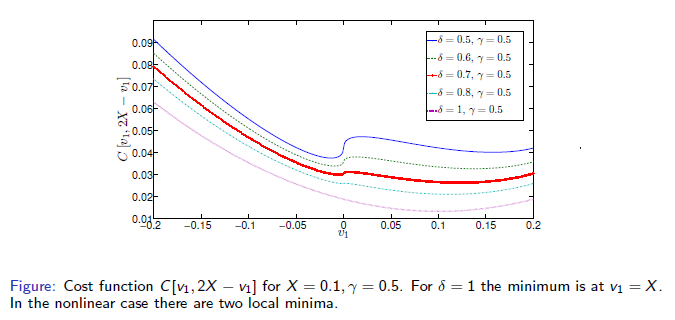
\includegraphics[width=0.6\textwidth]{picture/(20)perturbative_solution.png}
\end{center}
For buy program, strong nonlinearity is $\delta > 0.5$\\
Optimal strategies with the constraint $v\geq 0$:
\begin{center}
	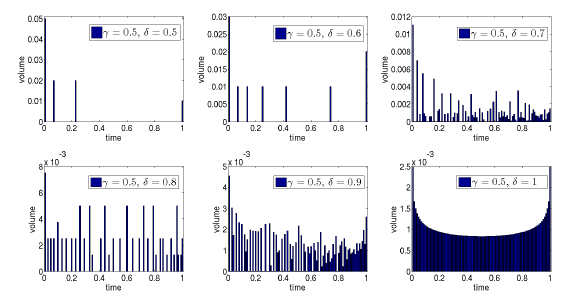
\includegraphics[width=0.6\textwidth]{picture/(21)perturbative_solution_constraint.png}
\end{center}
The optimal strategy is to trade in bursts separated by no trading periods (buy, wait price go down, buy again).\\
Not linear optimal buy: small intense bursting periods + long period call
\begin{center}
	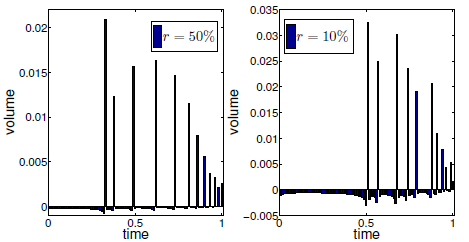
\includegraphics[width=0.6\textwidth]{picture/(22)spread_regularization.png}
\end{center}